\section{Overview}

Consider a group of connected UAVs deployed in a convex or non-convex environment. Convex environments consist in a domain without obstacles, while non-convex environments include  free-standing  obstacles  areas  with non-convex boundaries \cite{breitenmoser2010}. This work focuses on non-convex environments, where the obstacles are the surveillance radars, that we will call threats. Our approach, however, also applies for convex environments.

We consider that the UAVs are flying in constant altitude, therefore the environment can be represented by a bidimensional scenario composed by UAVs and threats. Moreover, we consider that each UAV is equipped with a radar responsible for communication. According to \cite{adamy2004}, in terms of signals frequency, communication signals are typically considered to be in the High Frequency (HF), Very High Frequency (VHF) or Ultra High Frequency (UHF). UAVs are able to communicate only with other UAVs within the same communication range. Given this communication topology, the collaborative UAV network can be represented by an undirected graph where each UAV is a vertex and each communication link between two UAVs is an edge of the graph. Figure \ref{fig:communicationLink} presents the communication topology in a collaborative UAV network.

\begin{figure}[hbt!]
      \centering            
      \subfloat[Disconnected newtork.]{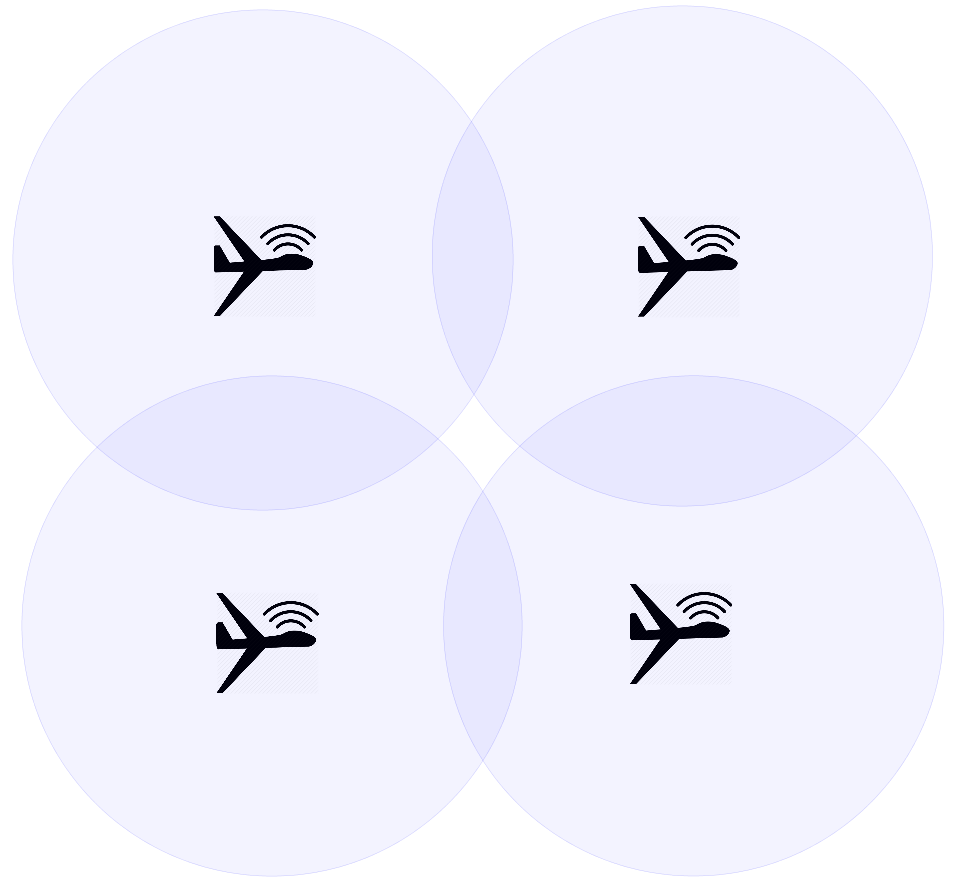
\includegraphics[width=0.35\textwidth]{Figures/conn1.png}} 
      \subfloat[Connected network.]{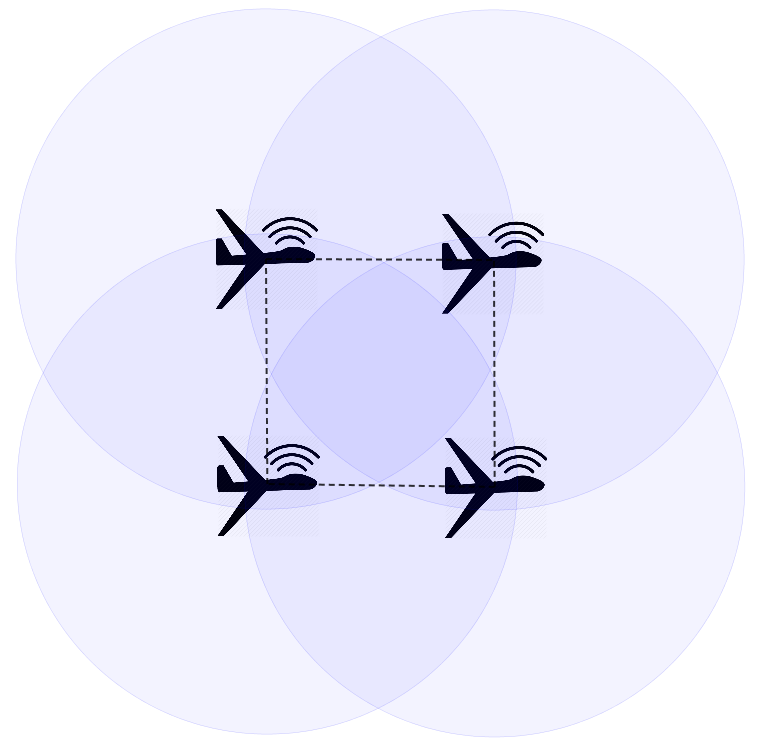
\includegraphics[width=0.35\textwidth]{Figures/conn2.png}}   \\ \centering
       \caption{Communication topology in a collaborative UAV network.}
    \label{fig:communicationLink}
\end{figure}


Threats are represented by circles, defined by their center position (physical radar position) and detection range. In order to respond to threats, the UAVs must be able to detect them during flight. Given that the threat range is normally larger than the detection range of an UAV, the detection of these radars is often given by passive receivers, which can be used to detect radar emissions over considerable distances \cite{gross_2007}. In this regard, we consider that the UAVs are equipped with Radar Warning Receivers (RWRs), which are able to detect the emissions from the threats. 

In this work, the UAV objective is to fly from the start position to a common goal position using a collaborative approach to detect and avoid threats, using an active stealth policy. To reproduce the scenario, we propose a simulation model over a time interval $t=[t_0..t_{max}]$. Since we do not consider lethal threats such as FCRs, all UAVs will achieve the goal. If all UAVs reach the goal before $t_{max}$, the mission is considered accomplished. A specific scenario consisting of UAVs performing collaborative tasks in hostile environments is presented in Figure \ref{fig:scenario}. In this figure, the threats are represented by the red circles.

\begin{figure}[h!]
    \centering
    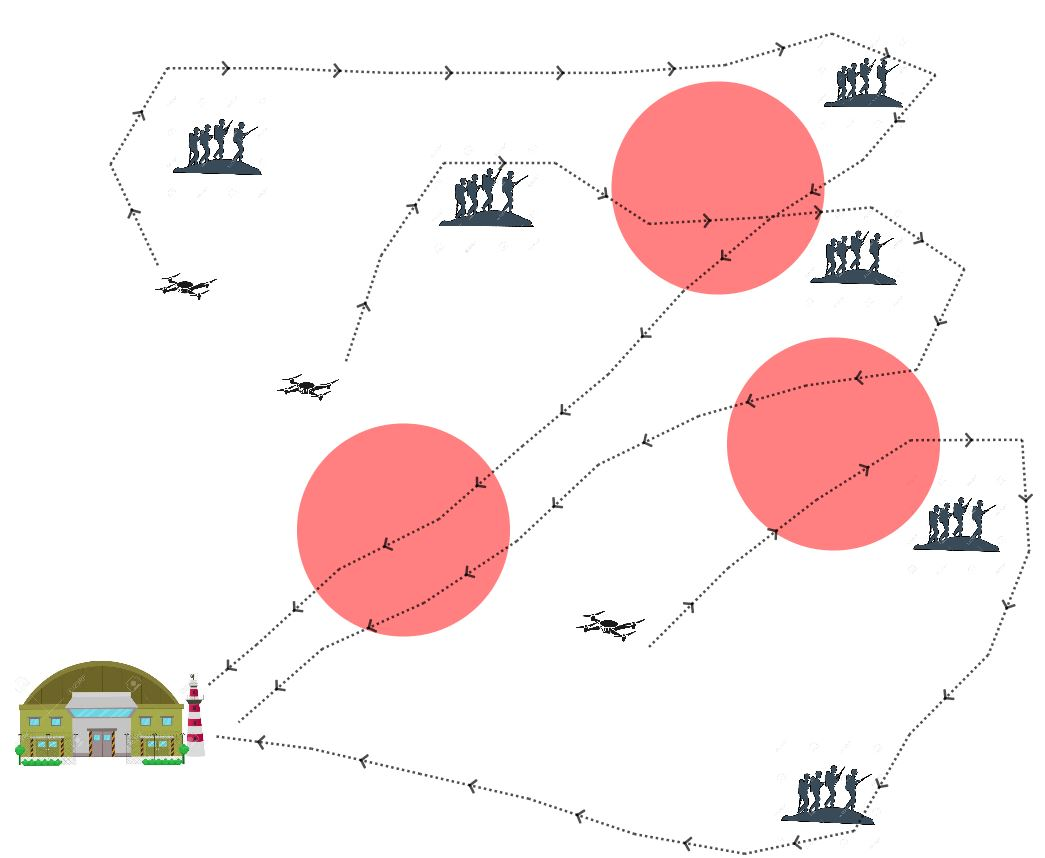
\includegraphics[width=0.6\textwidth]{Figures/scenario.png}
    \caption{An instance of the proposed scenario.}
    \label{fig:scenario}
\end{figure}

Notice that, for this scenario, the UAV network is fragmented into two local networks, since these networks are further from each other than the communication range of the UAVs. Moreover, these local networks are totally independent. There will only be collaboration between these two networks if at least one UAV of each of the networks communicates, thus unifying the networks. The remainder of this chapter details the proposed model. 

\section{Threat identification}

Due to the fact that our model considers that the detection of threats by the UAVs is passive, it is important to differentiate the concepts of detection range and detectability range. According to \cite{adamy2004}, a radar's detection range is the range at which it can detect a target, while the detectability range is the range at which its signal can be received and detected by a receiver.
 
This work is not focused on modelling electronic aspects of signals for the detection of a threat by the RWR or the detection of an UAV by a surveillance radar, but in modelling an stealth approach in collaborative UAV networks. Thus, the radar modelling is simplified as a range for detection. A threat is considered detected by an UAV if its range overlaps the RWR range, and an UAV is considered detected by a threat if the UAV is inside its detection range, as shown in Figure \ref{fig:rwr}. It is possible to notice that, in this case, the UAV is detecting the threat but the threat does not know about the presence of the UAV, because this is not in its detection range. 

\begin{figure}[h!]
\centering
\includegraphics[width=0.40\textwidth]{Figures/rwr.png}
\caption{Threat identification with RWR.}
\label{fig:rwr}
\end{figure}

Beyond the knowledge about the presence of a radar, when the RWR detects a threat, the detection range of this threat must be estimated so that other UAVs can avoid this region. The first step to estimate the threat region consists in calculating the electronic position of the threat. According to \cite{exercito_2009}, the electronic positions are commonly estimated by two different approaches: Direction Find (DF) and Time of Arrival (TOA). The DF is the technique used in most electronic localization systems due to low cost and simplicity. It analyses the direction of the emitted electromagnetic waves and can be implemented by two distinct processes:

\begin{itemize}
    \item \textbf{Horizontal localization:} The electronic position of the target is estimated by receivers and special systems of antennas that allow to establish the direction of the emissions. If measurements are made from properly spaced points, the intersection of these directions will indicate a probable area of the sender's location. This technique can be implemented using two approaches: using several UAVs, that detects a threat simultaneously or with a single equipment, performing azimuth measurements in successive positions. Figure \ref{fig:horizontalLoc1} shows an example of horizontal localization using different UAVs, while Figure \ref{fig:horizontalLoc2} presents an example of horizontal localization using a single UAV in different moments. 
        
    \begin{figure}[h!]
      \centering
      \subfloat[Using different UAVs.]{\includegraphics[width=0.4\textwidth]{Figures/eletronicLocalization1.png}\label{fig:horizontalLoc1}}
      \subfloat[Using a single UAV.]{\includegraphics[width=0.4\textwidth]{Figures/eletronicLocalization2.png}\label{fig:horizontalLoc2}}
      \caption{Horizontal localization.}      
    \end{figure}
    
    \item \textbf{Vertical localization:} The electronic position of the target is estimated by systems that use only one station to provide the coordinates of the opposing sender. In this technique, the direction of arrival and the height of the ionosphere are used to estimate the origin of the signal. This technique is only efficient for electromagnetic signals in the frequency range of HF, which suffer refraction in the ionospheric layer.
\end{itemize}

On the other hand, TOA consists in verifying the time between the electromagnetic pulses. This technique is more complex than DF, however it is more precise w.r.t. threat position estimation. If the exact moment at which the signal is emitted is known, for instance using an RWR, it is possible to estimate the threat's position. When the receptor detects the signal, a circumference is calculated with the distance between the receiver and the target. By intersecting two or more circles, it is possible to determine the location of the target \cite{exercito_2009}. In the same way that occur with Horizontal Location, this approach can be used by more than one UAV, as shown in Figure \ref{fig:DFOA1}, or using a single UAV in different moments, as shown in Figure \ref{fig:DFOA2}.

   \begin{figure}[h!]
      \centering
      \subfloat[Using different UAVs.]{\includegraphics[width=0.49\textwidth]{Figures/eletronicLocalization4.png}\label{fig:DFOA1}}
      \subfloat[Using a single UAV.]{\includegraphics[width=0.49\textwidth]{Figures/eletronicLocalization3.png}\label{fig:DFOA2}}
      \caption{Difference time of Arrival.}      
    \end{figure}

The exact moment at which the signal is emitted is sometimes unknown. Even in this case, it is also possible to estimate the radar location by Time of Difference Arrival (TDOA), which  is a technique based on the premise that any transmitted signal will arrive at different times in the receiver on the ground. From some mathematical analysis, it is possible to draw parabolas that will coincide at a certain point to determine the coordinates of the emitting target \cite{exercito_2009}.

This work does not intend to address the procedure of electronic localization and the error from position estimation. When an UAV detects the presence of a threat, it is assumed that the threat position is precisely known and its detection range can be calculated by:

\begin{equation}
R' = \sqrt{(P_x - P'_x)^2 + (P_x - P'_y)^2} - R,
\label{eq:threatRange}
\end{equation}

where $R$ is the RWR range of the UAV, $P'$ is the threat's position and $R'$ is its detection range.

Once we are considering that all the UAVs are equipped with an RWR, our model can uses a communication model based on intrusion detection described in \cite{farhan_2010}. Intrusion detection communication models can be classified into three groups:

\begin{itemize}
    \item \textbf{Standalone:} every node makes the detection without collaborating with others.
    \item \textbf{Distributed and Cooperative:} each node detects intruders as in the standalone approach, but communicate with other mobile nodes to exchange attack data for supporting global decisions making and agreeing on responses
    \item \textbf{Hierarchical:} the detection procedure is generally divided into small groups, such as clusters, and zones where some mobile nodes have more responsibility than others in the same group.

\end{itemize}

The Distributed and Cooperative is the model which most applies to our scenario. In our context the intruders are the threats. Based on this, every time an UAV detects a threat, a Depth-First Search procedure is applied in order to identify the UAVs that are connected to this node \cite{tarjan_1972}. These UAVs have their list of known threats updated and their path recalculated to avoid the new threat.

For stealthiness purposes, the UAVs that detect a threat cannot continue sharing information while in a critical area, otherwise the content of the communication could be heard by an passive radar. Thus, a safety distance must be added to the estimated threat range. At this moment, we are considering this new threat range as the union of the communication range of the UAV and the estimated detection range of the threat. We named this as \emph{Virtual Range} of the threat.

This approach is justified because we are assuming that the surveillance radars are in strategic locations, where it is essential to know the presence of enemy aircraft. Therefore, the probability of the presence of passive radars in this region is high, since some aircraft has some features that makes its detection harder by using surveillance radars. The UAVs may have different types of equipment, but for the collaborative approach adopted in this work, we consider that it is equipped with RWR and a communication radar. As the RWR is a signal receiver, it is not necessary to turn it off. Thus, the UAV will only turn the communication radar on again when the RWR does not detect the presence of any threat.  

\section{UAVs displacement model}

Given that each UAV state is its position $p_i\in\mathbb{R}^m$,  and \mbox{$p=\left[p_1^T\ldots p_N^T\right]^T\in\mathbb{R}^{N \times m}$} is the state vector of the multi-UAV system. Assume that each UAV can be modeled as a single integrator system and its velocity can be directly controlled, namely:

\begin{equation}
\dot{p}_i = u_i,
\label{eq:singleintegrator}
\end{equation}

where $u_i\in \mathbb{R}^m$ is a control input.

Consider a scenario where the UAVs must perform a mission using a collaboratively approach. Several factors must be taken into account in order to do so without compromising the success of the mission. For instance, the UAVs must avoid the enemy radars. Moreover, depending on the kind of mission, they must improve or decrease the coverage area, or improve the level of robustness to failures of the overall network. Based on this, the UAVs displacement can be modelled as a combination of control laws and adaptive gains. The combined control law for supporting the movement of UAV $u_i$  is then defined as:

\begin{equation}
u_i=\tau u_i^p + \sigma u_i^c + \rho u_i^r + \phi u_i^v
\label{eq:integratedcontroller}
\end{equation}

where: 

\begin{itemize}
    \item $u_i^p$ is the control law responsible for the the path planning and enemy radars avoidance.
    \item $u_i^c$ is the generalized connectivity maintenance control law;    
    \item $u_i^v$ is the control law responsible for improving the coverage area;
    \item $u_i^q$ is the control law responsible for improving the robustness to failures;    
    \item $\tau$, $\sigma$, $\rho$ and $\phi$ are the adaptive gains of the control laws.
\end{itemize} 

This work extends the combined control law model described in Ghedini \cite{ghedini_2017}, by increasing the path planning control law $u_i^p$. This displacement model is based on differential equations. Notice that if an adaptive gain is zero, its corresponding control law is inactive, i.e, the UAV does not need to change its position regarding the respective control law. The control laws are addressed as follows. For instance, considering a scenario in which the gain settings are $\tau=1$, $\sigma=75$, $\phi=1$ and $\rho=0$. In this case, each UAV must move trough the planned path to increase both its sensing area, without increasing its robustness to failure, while keeping the global network connectivity and avoiding collision with other UAVs.

There are different displacement models in literature, such as the described in He and Dai \cite{he_2013}. In this model, the movements of the UAVs are determined by optimization of factors under movement constraints with genetic algorithm.  A problem when using optimization models based on genetic algorithms is the computational cost for the model to converge. Considering that our scenario is very dynamic, where the drones need to recalculate their flight routes several times due to the detection of enemy radars, a model based on differential equations, such as described in Ghedini \cite{ghedini_2017}, ends up being more advantageous.

\subsection{Path trajectory control law $u_i^p$}
Flying towards the target the UAVs perform dynamic detection of the threats. Once a threat is detected, it is necessary to replan a trajectory to avoid this region. Each UAV autonomously calculates its own path. However, depending on the application, the UAVs should fly using different approaches. Thus, a procedure to define the goal position of UAVs using local information is necessary. This section presents the control law responsible for driving an UAV $u$ to follow a path that avoids the threat regions.

\subsubsection{Flight path approaches}

There are several flight formations for conventional airplanes, however some of them are not applicable to UAV scenarios because in the context of unmanned aircraft, there is no concept of a pilot's vision range. As aforementioned, this works consider that the sensing mechanisms usually present in UAVs are the radar for communication and the RWR. Therefore, the flight formation can only consider these.

Different kind of missions may require different formations. We consider two kinds: a structured flight formation that minimizes the exposure of UAVs to threats and a unstructured flight approach that add mechanisms that allows coverage control and robustness to failure improvement. We describe these approaches in what follows.

\subsubsection{Structured flight approach}

According to \cite{giulietti_2000}, in a typical flight formation there are the roles of leader and wingmen. In this context, the wingmen follow the trajectory of the leader, taking the other aircrafts as a reference to keep its own position in the formation. The leader's responsibility is to define the trajectory to the goal. In a rigid flying formation, inter-aircraft distances must be kept constant. 
 
In hostile environments, where the UAVs do not have information about the threat location, exposure should be reduced. In this sense, there is a flight formation, described in \cite{borges_2017}, named trail, that is used to air-to-ground attack on dangerous environments. Figure \ref{fig:trailFormation1} presents an example of the trail formation. The numbers above the UAVs correspond to their formation ranking ($id$). The UAV with $id$ $1$ is the leader of the connected component and responsible for calculating the trajectory to the goal, while the others are the wingmen, which always calculate the trajectory to the successor, i.e., the UAV that has $id = a -1$, where $a$ is the current UAV $i$. The problem with such formation is that the UAVs are not supported by any other UAV in formation, consequently, if one of them fails or is hit by an enemy, the UAV communication network can easily become disconnected.
  
\begin{figure}[ht]
\centering
\includegraphics[width=.45\textwidth]{Figures/trailFormation1.png}
\caption{Trail formation for UAVs.}
\label{fig:trailFormation1}
\end{figure}

For generating this formation, the UAV that is chosen to be the leader of a connected component of the network is the UAV that has the shortest path to the goal. The other UAVs' ranking are generated based on the length of their path to the leader: the closer an UAV is to the leader, the lower is its ranking position. The formation ranking, however, cannot be static because the connection between two UAVs may be lost. There are two reasons for connectivity loss between UAVs in the proposed scenario: the first one occurs because the distance between the UAVs are greater than its communication range. The second one is due to the fact that an UAV can turn off its communication radar. Thus, it is essential for the communication that these situations are detected so that UAVs take actions to reestablish the formation as quick as possible \cite{giulietti_2000}. 

Another possible scenario where it is necessary to update the flight formation is when there are two connected components that are close enough to be merged. For updating  a flight formation, the number of connected UAVs within a formation ranking $1$ is verified. If there are more than one, the leader will be the UAV with formation ranking $1$ that has the shortest path to the goal. We choose as leader the UAV with the shortest path to goal instead of the UAV that is closest to the goal because, since the scenario contains threats that must be avoided and it is not possible to ensure that the UAV that is closest to goal will reach the goal earlier. Figure \ref{fig:trailFormation0} presents an example of scenario where two flight formations are merged. There are two UAVs with $id=1$. The one that is below is closest to goal, however, due to the presence of threats, its path to the goal is longer than the path of the other UAV with $id=1$.

\begin{figure}[hbt!]
      \centering            
      \subfloat[Before merge formation.]{\includegraphics[width=0.35\textwidth]{Figures/trailFormation0.png}}      
      \subfloat[After merge formation.]{\includegraphics[width=0.35\textwidth]{Figures/trailFormation0_1.png}}
      \caption{Leader selection during a formation merging procedure.}     
      \label{fig:trailFormation0}
\end{figure}


The other UAVs rank indexes are updated based on their distance to the new leader, as previously described. Figure  \ref{fig:trailFaulExample1} illustrates a connectivity loss, while the resulting ranking reconfiguration is presented in \ref{fig:trailFaulExample2}. On the other hand, Figure \ref{fig:MergeFormations} illustrates how two flight formations are merged.

\begin{figure}[h!]
      \centering            
      \subfloat[Before fragmentation.]{\includegraphics[width=0.35\textwidth]{Figures/trailFormation2.png}\label{fig:trailFaulExample1}}      
      \subfloat[After fragmentation.]{\includegraphics[width=0.35\textwidth]{Figures/trailFormation3.png}\label{fig:trailFaulExample2}}            
      \caption{Connection fault example.}     
      \label{fig:trailFaulExample}
\end{figure}

\begin{figure}[h!]
      \centering            
      \subfloat[Start scenario.]{\includegraphics[width=0.35\textwidth]{Figures/trailMerge1.png}}      
      \subfloat[Update formation Id.]{\includegraphics[width=0.35\textwidth]{Figures/trailMerge2.png}}     \\
      \subfloat[Start move UAVs.]{\includegraphics[width=0.35\textwidth]{Figures/trailMerge3.png}}      
      \subfloat[Trail formation established.]{\includegraphics[width=0.35\textwidth]{Figures/trailMerge4.png}\label{fig:trailMerge4}}      
      \caption{Merge two formations in trail.}     
      \label{fig:MergeFormations}
\end{figure}

\subsubsection{Unstructured flight approach}

Using a structured flight approach, such as the trail, does not make possible to change the UAVs position for different tasks, for instance for coverage area improvement, as the formation can be undone. The unstructured flight approach we are using consider that each UAV will calculate its own path to the goal. Therefore, there is no leadership between UAVs. Figure \ref{fig:unstructuredFlightFormation} illustrates a scenario in which the UAVs are flying using an unstructured flight formation. 

\begin{figure}[ht]
\centering
\includegraphics[width=.45\textwidth]{Figures/unstructuredFormation.png}
\caption{Example of unstructured flight formation.}
\label{fig:unstructuredFlightFormation}
\end{figure}

There are different paths from a starting point to the goal using a non-deterministic algorithm for path planning such as RRT. In order to have a connected network, it is essential that the trajectories calculated by UAVs that are connected do not differ too much. In this context, it is possible to apply some curve similarity metric for evaluating how close two paths are in order to match them. There are several curve similarities metrics, two of them are the  Discrete Fr{\'e}chet Distance (DFD) and the Modified Hausdorff Distance (MHD).

The DFD is a variation of the Fr{\'e}chet distance for using with polygons. This metric searches for all coupling possibilities between the polygon end points. Given two curves $f:[a, b] \rightarrow V $ and $g:[a_r, b_r] \rightarrow V$, the distance $D$ can be calculated as follows \cite{eiter_1994}: 

\begin{equation}
D = \delta(f,g) = \inf_{\alpha, \beta \in [0,1]} max[f(\alpha(t)), g(\beta(t))]
\end{equation}

The MHD is a variation of the Hausdorff distance. For applying this distance to two curves $f:[a, b] \rightarrow V $ and $g:[a_r, b_r] \rightarrow V$ , it is necessary to build a distance vector ($v$) for $f$ and a distance vector ($vr$) for $g$. Then, given a point $x \in f$, each position of $v$ is defined as the minimum distance from $x$ to the points belonging to $g$. In addition, given a point $y \in g$, each position of $vr$ is defined as the minimum distance from $y$ to the points belonging to $f$. The MHD is the maximum value between the average of $v$ and the average of $vr$. The closer the DFD or the MHD between two paths are to 0, the closer the paths are.  Our model uses the DFD for evaluating the path similarity \cite{dubuisson_1994}.

We propose a matching procedure that consists in defining a reference path and, based on it, try to match the path of others UAVs to it. The first step to perform this procedure consists in finding the reference path. In this direction, the UAVs are grouped based on the similarity between their paths. If the DFD between two UAVs paths is less than a threshold, the UAVs are considered to belong to the same group. The reference path will be the path closest to the goal of the UAV that is inside the group with the large amount of UAVs. If there are two or more groups with the same amount of UAVs, the reference path will be the best candidate of those groups whose path is closest to the goal. The procedure of matching is iterative, as illustrated by the activity diagram in Figure \ref{fig:unstructuredFormationDiagram}. Figure \ref{fig:refPathMatching} presents the result of an application of the matching procedure. The current position of the UAVs are represented by the blue points, while the goal of the mission is represented by a red point. The black circles are the threats, with the continuous line constituting the detection range of the enemies radars, while the broken line represents the virtual range of the threat. Notice that all the paths become close to each other and, as a consequence, the likelihood of a network disconnection decreases, which is desirable for cooperative tasks.

\begin{figure}[hbt!]
\centering
  \includegraphics[width= 0.5\linewidth]{Figures/unstructuredFormation1.png}
  \caption{Activity diagram of the reference path matching procedure.} \label{fig:unstructuredFormationDiagram}
\end{figure}

\begin{figure}[hbt!]
      \centering            
      \subfloat[Before executing the path matching.]{\includegraphics[width=0.45\textwidth]{Figures/unstructuredFormation2.png}\label{fig:unstructured}}      
      \subfloat[After executing the path matching.]{\includegraphics[width=0.45\textwidth]{Figures/unstructuredFormation3.png}\label{fig:unstructured2}}
      \caption{Reference path matching example.}     
      \label{fig:refPathMatching}
\end{figure}

The procedure used for computing the flight path planning in both flight formation approaches is addressed as follows. 

\subsubsection{Flight path planning}

Since each UAV knows the position that it must reach to accomplish the mission, each of them calculates its own path to the goal. There are two situations for path planning: when an UAV is inside a threat region (communication radar is turned off), and when a UAV is outside a threat region. With regard to the algorithm for path planning, the difference between these scenarios depends on the definition of the goal position. By default, the goal position of the UAVs is influenced by the approach they are flying. In the case of the structured formation, the wingmen follow the leaders. On the other hand, by using the unstructured approach there is no leadership. All the UAVs calculate the paths directly to the goal of the mission. The case when an UAV is exposed to a threat will be addressed later.

Considering that RRT is a widely used technique for path planing with obstacle avoidance for UAVs, we use this algorithm as reference for computing the path planning. The Algorithm \ref{alg:rrt} shows how RRT computes the path planning from current position to a goal position. 

\begin{algorithm}
\caption{RRR algorithm - Compute path}\label{alg:rrt}
\begin{algorithmic}[1]
\Procedure{ComputePath}{$p_{current}$, $p_{goal}$, $p_{obstacles}$, $n_{edges}$, $e_{length}$, $n_{max}$} 
\State $G\gets Graph(p_{current})$ \Comment{Current position is the first vertex of the graph.}
\State $i\gets 1$
\State $k\gets 1$
\While{$k\leq=n_{edges} \And i\leq=n_{max}$}
\State $q_{rand}\gets CreateRandomPoint()$
\State $q_{near}\gets NearestVertex(q_{rand}, G)$
\State $q_{new}\gets TruncateEdge(q_{near}, q_{rand}, e_{length})$
\If{$\neg Intercept(q_{new}, p_{obstacles})$}
\State $G.addVertex(q_{new})$
\State $G.addEdge(q_{near}, q_{new})$
\State $k\gets k+1$
\EndIf
\State $i\gets i+1$
\EndWhile\label{euclidendwhile}
\State $p_{near}\gets ClosestVertexToGoal(G, p_{goal})$ \Comment{Get vertex that is closer to the goal}
\State $path\gets G.ShortestPath(1, p_{near})$
\State \textbf{return} $path$
\EndProcedure
\end{algorithmic}
\end{algorithm}

A limitation of RRT is not consider the movement constraints of the UAVs. Thus, we use an adaptation of this method for avoiding invalid movements based on angle validation. RRT has as inputs a start point $p_0$, the number of branches $n_e$ and a distance $d$. The initial tree contains only $p_0$. Then, a random position in the scenario is generated and the nearest node $k_n$ to this position in the tree is searched. Once the node is identified, a line $l$ that passes along these two nodes is generated. Next, a line segment of length $d$, starting from $k_n$, is extracted from $l$. If the line segment does not pass thought any forbidden region (zone around a threat, in our case), this branch is added to the tree. This process is repeated until the number of branches is equal to $n_e$ or when the number of iterations is greater than a threshold. Taking into account that there is no guarantee that RRT will provide a feasible path to the goal, the UAVs will always move towards the nearest position of the goal $p_f$, considering the tree generated by RRT. The shortest path between the start position and $p_f$ is computed using the Dijkstra algorithm \cite{dijkstra_1959}.  The resulting tree is highlighted in Figure \ref{fig:rrt1}. 

\begin{figure}[hbt!]
\centering
\includegraphics[width=.7\textwidth]{Figures/rrt1.png}
\caption{Path generated by RRT.}
\label{fig:rrt1}
\end{figure}

\subsubsection{Angle validation}

Since it is more important for the present model to evaluate the behavior of the UAV network according to a stealth policy and a combined control law and not modeling a large set of handling dynamical restrictions, such as yaw and pitch angles, described in \cite{he_2013}, we adopt a single handling constraint, which is the angle variation between movements.

Every time a UAV moves from position $P_1$ to a new position $P_2$ the angle between these points is calculated. The equation for calculating the angle $\epsilon$ between  $P_1$ and $P_2$ is described by:

\begin{equation}
    \epsilon = atan2(y,x), 
\end{equation}

where $y$ is the difference between the y-axes value of $P_1$ and $P_2$ and $x$ is the is the difference between the x-axes value of $P_1$ and $P_2$. The function $atan2(y,x)$ is the function $tan^{-1}(\frac{y}{x})$, limiting the resulting angle in the range of $[-pi, pi]$.

For avoiding invalid movements, an UAV movement will only be considered valid if the angle generated by the new and current positions is in a specific range, as illustrated in Figure \ref{fig:flightAngle}. In this figure, the UAV flights from position $P_{i-1}$ to $P_i$. The angle between $P_i$ and the next movement must not exceed the max angle variation $\theta$, otherwise it will be considered an invalid movement.

\begin{figure}[hbt!]
\centering
\includegraphics[width=.6\textwidth]{Figures/angleVariation.png}
\caption{Angle validation of UAV movement}
\label{fig:flightAngle}
\end{figure}

In terms of implementation, a solution to use this approach is to adapt the RRT algorithm to only generate branches of the tree if the angle generated by the new intermediate goal point and the nearest node in the tree is in a specific range. Figure \ref{fig:pathWithAngleRestriction} presents the resulting branches (black lines) and the path generated by the execution of RRT (green lines) with and without angle restrictions for different values of $\epsilon$. The red circles represents the threats.

\begin{figure}[hbt!]
      \centering            
      \subfloat[Resulting path with $\epsilon$ = 90$\degree$. ]{\includegraphics[width=0.45\textwidth]{Figures/rrt90.PNG}}      
      \subfloat[Resulting path with $\epsilon$ = 60$\degree$.]{\includegraphics[width=0.45\textwidth]{Figures/rrt60.PNG}}  \\ \centering
      \subfloat[Resulting path with $\epsilon$ = 45$\degree$.]{\includegraphics[width=0.45\textwidth]{Figures/rrt45.PNG}} \caption{Generated path with angle validation.}
      \label{fig:pathWithAngleRestriction}     
\end{figure}

\subsubsection{Path reduction}

Since the output of RRT is a set of consecutive lines, it is possible to optimize the path to reduce its length. This procedure consists in attempting to trace the longest lines as possible between path vertexes. Figure \ref{fig:pathReduce} illustrates an example of the path reduction procedure, notice that it significantly changes the original path provided by RRT. It is important to note that the new lines are restricted to the valid angle range condition aforementioned.

\begin{figure}[hbt!]
\centering
\includegraphics[width=0.9\textwidth]{Figures/RRT_Reduce.png}
\caption{Path reduction example.}
\label{fig:pathReduce}
\end{figure}

The result of the procedure to reduce paths provides a path where the vertices are located at varying distances. The UAV needs to move by following the path according to a reference speed, then it is necessary to know the position that the UAV would be at the moment $t$ within the previously computed path. Thus, by using interpolations, new equidistant vertexes are generated \cite{davis_1975}. The distance between them is proportional to the speed of the UAV.

\subsubsection{Path smoothing}

RRT provides, as output, a linear piecewise representation of the trajectory. Thus, it may be necessary to apply a path smoothing method for generating feasible trajectories, as highlighted in \cite{borges_2016}. The smoothing procedure considered here is based on an algorithm proposed to perform horizontal segmentation of highways \cite{coelho_2015}. The first step of this algorithm consists of identifying the instant that the angular coefficient varies, as shown in Figure \ref{fig:pathSmoothing1}. Given these moments, a set of neighbours are selected, as presented in Figure \ref{fig:pathSmoothing2}. 

\begin{figure}[h!]
      \centering            
      \subfloat[Detection of angular coefficient variation.] {\includegraphics[height=0.35\textwidth,width=0.45\textwidth]{Figures/PathSmoothing1.eps}\label{fig:pathSmoothing1}}      
      \subfloat[Derfining in neighbourhood.]{\includegraphics[height=0.35\textwidth,width=0.45\textwidth]{Figures/PathSmoothing2.eps}\label{fig:pathSmoothing2}}  \\ \centering
      \caption{Angular coefficient variation detection.}
\end{figure}

Taking into account the set of computed points, a circle is fit \cite{coope_1993}, resulting in the radius and center coordinates of the circle that best adjust to the set of points, as shown in Figure  \ref{fig:pathSmoothing3}. Computed the circle fitting, it is necessary to select the points in the circles that correspond to the points of the neighborhood used for fitting, as presented in Figure \ref{fig:pathSmoothing4}. 

\begin{figure}[h!]
      \centering            
      \subfloat[Circle fitting.]{\includegraphics[height=0.35\textwidth,width=0.45\textwidth]{Figures/PathSmoothing3.eps}\label{fig:pathSmoothing3}}      
      \subfloat[Select points in circles.] {\includegraphics[height=0.35\textwidth,width=0.45\textwidth]{Figures/PathSmoothing4.eps}\label{fig:pathSmoothing4}}  \\ \centering
      \caption{Circle fitting procedure}
\end{figure}

The next step consists in replacing the neighbourhood points by the points in the generated circles, as shown in Figure \ref{fig:pathSmoothing5}. Finally, a moving average procedure is executed in order to match lines and curve regions \cite{azami_2012}. Figure \ref{fig:pathSmoothing6} illustrates the path after the execution of successive moving average procedures.

\begin{figure}[h!]
      \centering            
      \subfloat[Replacing points in neighbourhood] {\includegraphics[height=0.35\textwidth,width=0.45\textwidth]{Figures/PathSmoothing5.eps}\label{fig:pathSmoothing5}}      
      \subfloat[Path after moving average procedure.] {\includegraphics[height=0.35\textwidth,width=0.45\textwidth]{Figures/PathSmoothing6.eps}\label{fig:pathSmoothing6}}  \\ \centering
      \caption{Path after path smoothing procedure.}
\end{figure}

\subsubsection{Computing the goal for an UAV in a threat region}

The stealth policy of turning off the communication radar adopted here consider that the UAV that enters a threat region cannot communicate with other UAVs. Moreover, the UAV must trace a path to leave the area of the threat. In this sense, there are two approaches for computing the goal, which is used as reference for path planning, to leave the threat region: the first one implies leaving the threat region quickly, while the other approach consists in computing the goal position in a region that the other UAVs of the formation will possibly pass through, thus improving the chance for the UAV that turned off the radar to regroup with the others.

The procedure for computing a goal for the UAV in a threat region assumes that each UAV knows its own position $p_i$ and its neighbor positions $p_{\mathcal{N}_i}=\{p_j,\forall j\in\mathcal{G}: i,j \in \mathcal{E}\left(\mathcal{G}\right)\}$.

The first step consists in generating candidate points that allows the UAV to leave the threat region. An UAV has two candidate points $P_i'$ and $P_i''$, one at each direction. These points are obtained from the equation of the line $L_{Proj}$ that passes through the last position of the UAV $P_{i-1}$ and its current position $P_i$. The candidate points  $P_i'$ and $P_i''$ are the first points that are outside the threat, considering the line $L_{Perp}$ which is perpendicular to $L_{Proj}$ and pass through the center of the threat. Figure \ref{fig:LeaveThreat1} illustrates the procedure to compute the candidate points.

\begin{figure}[hbt!]
\centering
\includegraphics[width=0.65\textwidth]{Figures/leaveThreat1.png}
\caption{Candidate points for computing path planning to leave threat region}
\label{fig:LeaveThreat1}
\end{figure}

The next candidate point $P_i'''$ results from the estimation of future positions of connected UAVs. While in the trail formation, we have the leader and the wingmen, in the unstructured approach there is no leadership. Therefore, the procedure for estimating the future position of UAVs is different for these flight formation approaches and are described as follows.

\subsubsection{Trail formation}

The procedure for estimating the future position of the UAVs flying using the trail formation is straightforward. The UAV that is exposed to a threat will compute the path to the goal, considering that is in the last position of its successor into the flight formation. 

RRT it is not a stochastic algorithm, thus it is not ensured that the path of the successor and the estimated path will coincide. On the other hand, because of threat avoidance, the angle validation and the path reduction procedure, the chance of these paths coinciding is high. The estimated path position $P_i'''$ is the point in the computed path that is closest to the previously computed candidates $P_i'$ and $P_i''$, as shown in Figure \ref{fig:LeaveThreat2}.

\begin{figure}[h!]
\centering
\includegraphics[width=0.8\textwidth]{Figures/leaveThreat2.png}
\caption{Candidate points for computing path planning to regroup with the other UAVs.}
\label{fig:LeaveThreat2}
\end{figure}

\subsubsection{Unstructured flight approach}

Considering that there is no leadership in the unstructured flight approach, it is not possible to estimate the future position of UAVs by computing the path of an UAV's successor in formation. Thus, it is necessary to consider the paths of all UAVs that are connected with the UAV that turned off the communication radar

The UAV that is exposed to a threat will compute the paths to the goal of all its neighbours. Thus, the UAVs are clustered based on the DFD between their computed paths. Whether the DFD between two UAVs' paths is lower than a threshold, these are considered belonging the same group. A large amount of UAVs in the same group indicates that the most part of UAVs tends to fly using a nearby path. Therefore, the chance of estimating correctly the future position of the UAVs increases. In this direction, considering that maybe exist more than a group with the same amount of UAVs, for each path in the groups with the most amount of UAVs, the points $P_i^j$ that are close to the previously computed candidates $P_i'$ and $P_i''$ are selected. 

The next step consists in compute the average point $P_i^javg$ for each previously computed points $P_i^j$. Then, the estimated path position $P_i'''$ is the point $P_i^javg$ which results int the shortest path length between current UAV position and $P_i^javg$. By using this approach, we improve the chance of the UAV reconnect with other uavs due to the fact that we drive the UAV to a position in which the most UAVs of the network will probably pass near.

\subsubsection{Selection of the best candidate point}

Once the candidate points $P_i'$, $P_i''$ and $P_i'''$ were computed, it is necessary to establish the criterion for which candidate point should be the goal of the UAV. If $P_i'''$ exists\footnote{$P_i'''$ can only be computed in the case that the UAV is connected to another UAV.}, this point is outside a threat region and the path length from the current UAV position to $P_i'''$ does not exceed a maximum length threshold $L_{max}$, this candidate point is selected to be the goal. Otherwise, the choice is between $P_i'$ and $P_i''$. Thus, the goal is the candidate that is outside a threat region, whose path length between the current UAV position and these two candidate points is smaller. 

Notice that if there is no candidate point that meets the constraints, for instance in the case of all candidates inside threat regions, the goal that supports the path planning to leave the threat region will be the goal of the mission. However, in order to avoid flying over the physical position of the radar (center of threat region), the path planning consider the threat range to be lower than it actually is, making the UAV fly across the edges of the detection range. 

\subsubsection{Displacement model}

The objective of this control law is to drive the UAV $u$ to follow a path that avoids the threat regions, given a path $Path\gamma(u)$ of the UAV $u$, located at the position $p_i$ at a moment $t$. By using interpolation, it is possible to estimate the position $x_\gamma^i$ in which the UAV should be at a moment $t+1$, following $Path\gamma(u)$. Notice that the distance from positions $p_i$ and $x_\gamma^i$ is  parameterized and impacts the speed of the UAV in our model. Thus, the control law that drives the UAV $u$ to follow the path planning is defined by:

\begin{equation}
u_i^p = \tfrac{x_\gamma^i - p_i}{\left\| x_\gamma^i - p_i \right\|}\beta\left(t\right),
\label{eq:controllawPathPlanning}
\end{equation}
where $\beta\left(t\right)\in\mathbb{R}$ is the linear velocity of the UAVs.

Due to the performance purposes the path planning algorithm does not have to be executed at each iteration $t$. For instance, considering a scenario where the UAV $u$ does not shut down its communication radar and that the straight segment that passes through $p_i$ and $x_\gamma^i$ does not intercept any threat regions, and the generated angle between $p_i$ and $x_\gamma^i$ is within the range $\theta$, instead of running RRT again it is possible to update the previously computed path. The case in which the UAV is inside a threat region is analogous. However, when the UAV turns on the communication radar again, the path needs to be recalculated.

In this sense, before performing the RRT algorithm, the proposed model always verifies if it is possible to trace a line from the current position of the UAV to the goal position without passing through any threat, considering the angle validation constraint. This approach reduces the overall execution time, since the path planning algorithm does not need to be computed all the time.

\subsection{Connectivity maintenance control law $u_i^c$}

In order to guarantee the connectivity of a network, \cite{sabattiniijrr2013} propose an approach to solve the connectivity maintenance problem in a decentralized manner, using the algebraic connectivity property. For this purpose, consider a weighted graph, where the edge weights $w_{ij}$ are defined as follows:
\begin{equation}
w_{ij}=\left\{
\begin{array}{ll}
e^{-\left(\left\|p_i-p_j\right\|^2\right)/\left(2\sigma^2\right)}&\mbox{if }\left\|p_i-p_j\right\|\leq R\\
0&{otherwise.}	
\end{array}\right. 
\label{eq:edgeweightIJRR}
\end{equation}
where $e^{-\left(R^2\right)/\left(2\sigma^2\right)} = \Delta$, and $\Delta$ is a small predefined threshold. Notice that the definition of the edge weights introduces a discontinuity in the control action. However this can be avoided introducing a smooth bump function, as in \cite{do2008}. 

Define $\epsilon>0$ to be the desired lower-bound for the value of $\lambda$. The control strategy is then designed to ensure that the value $\lambda$ never goes below $\epsilon$. As in~\cite{sabattiniijrr2013}, the following energy function can then be utilized for generating the decentralized connectivity maintenance control strategy:
\begin{equation}
V\left(\lambda\right)=\left\{
\begin{array}{ll}
\coth \left(\lambda - \epsilon\right)\,\, & \mbox{if } \lambda>\epsilon\\
0 & \mbox{otherwise.}
\end{array}\right.
\label{eq:totaltensionCDC}
\end{equation}
The control design drives the UAVs to perform a gradient descent of $V\left(\cdot\right)$ in order to ensure connectivity maintenance. Considering the dynamics of the system introduced in~\eqref{eq:singleintegrator}, the control law is defined as: % follows:
\begin{equation}
{u}_i=u_i^c = -\tfrac{\partial V\left(\lambda\right)}{\partial p_i}=-\tfrac{\partial V\left(\lambda\right)}{\partial \lambda}\tfrac{\partial \lambda}{\partial p_i}.
\label{eq:Kfunction}
\end{equation}

\subsubsection{Collision avoidance}

The connectivity maintenance framework can be enhanced to consider additional objectives. In particular, as shown in~\cite{robuffogiordano2013}, the concept of generalized connectivity can be utilized for simultaneously guaranteeing connectivity maintenance and collision avoidance with environmental obstacles and among the UAVs. This is achieved considering the following generalized edge weights:

\begin{equation}
\omega_{ij} = w_{ij}\gamma_{ij},
\label{eq:generalizedweights}
\end{equation}
$\forall i,j = 1, \ldots, N$. In particular, the edge weights $w_{ij}$ represent the standard connectivity property. The multiplicative coefficients $\gamma_{ij}$ represent the collision avoidance edge weights, which have the following properties, $\forall i,j=1, \ldots, N$:

\begin{enumerate}
        \item $\gamma_{ij}=\gamma_{ij}\left(\left\|p_i-p_j\right\|\right)\geq0$. \label{property:cweights1}
		\item $\gamma_{ij}=0\,\,\,\mbox{if }\left\|p_i-p_j\right\| = 0$, and $\gamma_{ij}=1\,\,\,\mbox{if }\left\|p_i-p_j\right\| \geq d_{s}$. \label{property:cweights2}
		\item $\gamma_{ij}\left(d\right)$ is non-decreasing w.r.t. its argument $d$.\label{property:cweights4}
\end{enumerate}

where $d_s>0$ represents the safety distance. 

\subsubsection{Displacement model}



From the generalized edge weights $\omega_{ij}$ in~\eqref{eq:generalizedweights}, 
it is possible to compute the generalized Laplacian matrix $\mathcal{L}^G$, whose second smallest eigenvalue $\varphi$ represents the generalized connectivity of the graph. As shown in~\cite{robuffogiordano2013}, guaranteeing positiveness of the generalized connectivity $\varphi$ simultaneously guarantees maintenance of the algebraic connectivity 
and collision avoidance. This can then be achieved using the control law~\eqref{eq:Kfunction} replacing $\lambda$ with $\varphi$, namely:
\begin{equation}
{u}_i=u_i^c = -\tfrac{\partial V\left(\varphi\right)}{\partial p_i}=-\tfrac{\partial V\left(\varphi\right)}{\partial \varphi}\tfrac{\partial \varphi}{\partial p_i}.
\label{eq:genconnmaint}
\end{equation}

Since $\varphi$ and its gradient are global quantities, the proposed control law is centralized. A decentralized implementation can be achieved replacing $\varphi$ and its gradient with their estimates, computed by each UAV in a decentralized manner applying the procedure proposed in~\cite{sabattiniijrr2013}.
 \label{sec:connectivity}

\subsection{Improve coverage area control law $u_i^v$}

According to \cite{sangwan_2015} coverage can be defined as how well or to how much extent each point of a deployed network is under the vigilance of a sensor node. The coverage mechanism in the context of this work aims to improve the capacity of a UAVs of monitoring the environment, reducing the redundant areas and avoiding "holes" in the network. 

Ghedini \cite{ghedini_2017} describes a local model that uses a control law that improves the coverage area of multi-robot systems. In addition, it also shows how this control law operates in combination with control laws for connectivity maintenance and robustness to failures. The procedure is based on a Voronoi tesselattion, which is a widespread technique that supports several context of application approaches \cite{breitenmoser2010}. This control law is discussed in what follows.

\subsubsection{Voronoi coverage}

A Voronoi tessellation is a subdivision of a plane into cells based on the proximity of a set of points (named sites).
Let $P=\left[p_1,p_2, \ldots, p_n\right]$ be a set of points in the plane. Define $V(i)$, the Voronoi cell for $p_i$, to
be the set of points $q$ in the plane that are closer to $p_i$ than to any other site. Thus, the Voronoi cell for  $p_i$ is defined by 

\begin{equation} \label{eq:VoronoiDefinition}
V(i)=\{q \mid \|p_iq\| < \|p_jq\|, \forall j\neq i \}, 
\end{equation}
where  $\|pq\|$ denotes the Euclidean distance between points $p$ and $q$ \cite{mount_2002}.

According to Schawager \textit{et al.} \cite{schwager_2007}, if each point is positioned at the centroid of its Voronoi cell,  a cost function representing the sensing cost of a network is locally minimized.

Due to the requirements demanded by the defined scenario features, such as using local information, the strategy for modeling the Voronoi coverage is based on a local mechanism presented in \cite{breitenmoser2010}, described as follows. Let $V(i)$ be the Voronoi cell corresponding to a UAV located at $p_i$. A team of $n$ UAVs at positions $P= [p_i]_{i=1}^n\in\mathbb{R}^{Nn}$ navigate in a bounded polygonal environment $\Omega\Rightarrow\mathbb{R}^{N}$, where $\Omega$ is a closed set with the boundary $\partial\Omega$. 
Given  a positive density function $ \phi:\Omega\rightarrow\mathbb{R} >0$, the centroid of $V(i)$ is defined as

\begin{equation} \label{eq:centroidalVoronoi}
\mathit{C}_{V_i}=\frac{1}{{M}_{V_i}}\int_{V_i} \mathit{x} \, \phi(x)\mathrm{d}\mathit{x},
\end{equation}
where ${M}_{V_i}$ is the cell mass  \cite{breitenmoser2010}: 
\begin{equation} \label{eq:mass}
{M}_{V_i}=\int_{V_i} \phi(x)\mathrm{d}\mathit{x}.
\end{equation}

An optimal distribution of generating points implies that each of them is at the center of mass of its cell, i.e., $p_i = C_{V_i}, \forall i \in \{1,\dots,n\}$. This centroidal Voronoi tessellation (CVT) is a minimum-energy configuration in the sense that it minimizes the distance between points: 

\begin{equation} \label{eq:costVoronoi}
\mathscr{H}(P)=\sum_{i=1}^{n}\mathscr{H}(p_i) = \, \sum_{i=1}^{n}\int_{V_i} f(D(\mathit{p_i},\mathit{x})) ,\ \phi(x)\mathrm{d}\mathit{x},
\end{equation}

where $D(.)$ is the distance between a point $p_i$ and a location $x$ in $\Omega$, and $\phi(.)$  is the density function that describes the importance of different areas in $\Omega$ \cite{breitenmoser2010}. Considering the euclidean distance $D(p_i,x)=\|x-p_i\|$ as the distance function in~\eqref{eq:costVoronoi}:
\begin{equation} \label{eq:distancepartial}
\frac{\partial\mathscr{H}(p_i)}{\partial(p_i)}=-M_{V_i}(\mathit{C}_{V_i}-p_i)=0,
\end{equation}
the local minima is reached with a CVT since $\mathit{C}_{V_i}=p_i$ implies $\frac{\partial\mathscr{H}}{\partial(p_i)}=0, \forall i \in \{1 \dots n\}$.

The Voronoi coverage presented in \cite{breitenmoser2010} is based on the Lloyds algorithm \cite{du_2006}, which is a well-stabilished method for generating a centroidal Voronoi tessellation. It encompasses:    
\begin{enumerate}
	\item Create the Voronoi diagram for generating points $P$.
	\item Compute the centroid $[\mathit{C}_{V_i}]_{i=1}^n$ of each Voronoi cell.
	\item Set the new target position of each UAV as the centroid of its cell\footnote{Notice that the exposure to threats needs to be reduced in our model, thus, case the  centroid of its cell is inside a threat region, the UAV does not move in this direction.}.	 
\end{enumerate}
This process iterates until the computed centroids and the generating points are at the same positions. From the proportional control law  
~\eqref{eq:distancepartial} the simple first-order dynamics can be derived:
\begin{equation} \label{eq:derivatepartial}
u_i = u_i^v=\dot{p}_i=-\frac{k}{M_{V_i}}\frac{\partial\mathscr{H}(p_i)}{\partial(p_i)}=k(\mathit{C}_{V_i}-p_i).
\end{equation}

The procedure for locally computing the Voronoi cells assumes that each UAV knows its own position $p_i$ and its neighbor positions $p_{\mathcal{N}_i}=\{p_j,\forall j\in\mathcal{G}: i,j \in \mathcal{E}\left(\mathcal{G}\right)\}$. Thus, each UAV $i$ computes its local Voronoi ($V(i)$ Eq. \eqref{eq:VoronoiDefinition}). Having its voronoi cell $\mathit{C}_{V_i}$, the mass of the centroid is calculated (\eqref{eq:centroidalVoronoi}). Finally, to improve the coverage area, the UAV flight toward the mass of its cell centroid $\mathit{C}_{V_i}$.

The procedure for improving the coverage area iterates until a centroidal Voronoi tessellation is achieved or as it is convenient for the applicatio. The Voronoi tessellation and the mass of the centroid are recomputed at each $t$ seconds, setting according to the application requirements. If a UAV $i$ is at the centroidal position of its Voronoi cell, the weight for $u_i^v$ is zero, i.e., the $i$  UAV does not need to improve its position regarding coverage. 

This approach imposes some constraints to the scenario adopted here: the  procedure for creating a Voronoi tessellation generates some unbounded cells, being that for computing the mass of the centroid for a cell it needs to be bounded. Therefore, it is necessary to define a procedure to delimitate the unbounded cells. This issue is addressed as follows.

\subsubsection{Unbounded Voronoi tessellations}

Considering that the coverage approach is based on the generation of each cell centroid, the main issue of using the Voronoi tessellation as a means of improving the network coverage area is the treatment of unbounded cells.

A possible approach is addressed in \cite{sang_2015}. It focuses on presenting geographic data through Voronoi diagrams without having to specify a bounding box. However, the same procedure can be applied for bounding a Voronoi diagram with the advantage of using the UAV communication range for reducing the size or bounding cells, as the technique relies on defining a maximum size for a cell.

Figure \ref{fig:voronoi} illustrates a Voronoi cell for a generating point and a circle that defines the cell limits. 
\begin{figure}[ht] \centering
	\includegraphics[width= 0.30\linewidth]{Figures/voronoi.png}
	\caption{Mapping edges in a Voronoi Cell \cite{sang_2015}.}
	\label{fig:voronoi}	
\end{figure}
 
 All possible state classifications and actions for an edge can be visualized in this example. Each edge may:
 
 \begin{itemize}
	\item lay completely inside the bounding circle (edge A): it must not change;
	\item lay completely outside the bounding circle (edge C): it must be replaced by its corresponding circle;
	\item have one intersection with the bounding circle (edges B and E): the part laying inside the circle remains unchanged, the rest is replaced by its corresponding circle part;
	\item have two intersections with the bounding circle (edge D): it part laying inside the circle remains unchanged, the other two parts are replaced by their corresponding circle part.
\end{itemize}

The first step is to verify if a cell lies inside the bounding circle by computing the distance of each of its vertices to the circle center (in this application, the UAV position) and comparing it with the circle radius:
\begin{equation} \label{eq:distance}
distance_{(P,Center)} = \sqrt{(P_x-Center_x)^2 + (P_y-Center_y)^2},
\end{equation}
where $P_x$ and $P_y$ are the coordinates of each Voronoi cell point and $Center$ is the center point of the circle.

For those vertices that are completely outside the bounding circle (edge $C$ - Figure \ref{fig:voronoi}), its $x$ and $y$ coordinates are mapped to the circle point, i.e., the distance from the new point to the $Center$ is equal to the predefined radius:
\begin{equation} \label{eq:newPx}
NewP_x = Center_x + (P_x-Center_x) * Radius/distance(P,Center),
\end{equation}
\begin{equation} \label{eq:newPy}
NewP_y = Center_y + (P_y-Center_y) * Radius/distance(P,Center).
\end{equation}

For cutting the edges intersecting the circle (edges $B$,$D$ and $E$ - Figure \ref{fig:voronoi}), a straight line corresponding to an edge is computed: 
\begin{equation}
\begin{aligned}\label{eq:lineEdge}
y &= a*x+b \;when\; x_1 \neq\ x_2, a=(y_2-y_1)/(x_2-x 1 ) \;and\; b=(y_1 *x_2-y_2*x_1)/(x_2-x_1) \\
x &= a*y+b \;when\; x_1 = x_2, \; a=0 \;and\;  b=x_1, 
\end{aligned}
\end{equation}
where $(x_1,y_1)$ and $(x_2,y_2)$ are the coordinates of the two vertices. Then, the definition of the bounding circle is given by:
\begin{equation} \label{eq:boundingCircle}
y = Center_y \pm \sqrt{Radius^2 - {(x-Center_x)^2}} \; if \;  Radius^2 \geq  {(x-Center_x)^2}.
\end{equation}

The equations \eqref{eq:lineEdge} and \eqref{eq:boundingCircle} are then combined to find the intersections:  
\begin{equation} \label{eq:combiningEq}
Center_y \pm \sqrt{Radius^2 - {(x-Center_x)^2}} \; = \;  a*x+b.
\end{equation}
Solving equation \eqref{eq:combiningEq} in order to achieve a quadratic equation of the form  
$A*x^2+B*x+C=0$:
\begin{align}
A&=-1-a^2 \nonumber \\
B&=2*Center_x-2*a*(b-Center_y) \nonumber \\
C&=Radius^2-Center{_x}{^2}-(b-Center_y)^2, \nonumber\\
\end{align}
the values of $x$ are given by the general quadratic equation 
$x=-B\pm \sqrt{B^2-4*A*C}$, and the values of $y$ by equation \eqref{eq:lineEdge}. Thus, $x$ and $y$ determine the new cell boundaries. The computational complexity is $\mathcal{O}(n)$, where $n$ is the number of edges in the Voronoi diagram \cite{sang_2015}.  

\subsubsection{Displacement model}

The objective of this control law is to drive an UAV  to a position that increases the coverage area of the network. Thus, given an UAV $u$, located at position $p_i$, and its corresponding voronoi cell centroid $x_y^i$, the control law that drives the UAV to improve the coverage area can be defined as:

\begin{equation}
u_i^c = \xi_i\tfrac{x_\gamma^i - p_i}{\left\| x_\gamma^i - p_i \right\|}\delta\left(t\right),
\label{eq:controllawCoverage}
\end{equation}
where $\delta\left(t\right)\in\mathbb{R}$ is the linear velocity of the UAVs.

By default, $\xi_i=1$. However, considering that the exposure to threats needs to be reduced in our model, in case the Voronoi cell centroid of the UAV $u$ is inside a threat region, it does not move in this direction. In this case, we set $\xi_i=0$.

\subsection{Robustness to failures $u_i^r$}
Considering that failures of nodes playing a central role in the network communication are likely to affect most its connectivity --- and thus, the cooperation between UAVs, Ghedini \cite{ghedini_2016} addresses a way to improve the robustness of a local network to failures. This approach is defined by three execution steps, described as follows:

\begin{itemize}
    \item Evaluation of robustness of the network.
    \item Local evaluation of vulnerability of the nodes.
    \item Driving vulnerable UAVs to improve the robustness of the network.
\end{itemize}

\subsubsection{Robustness level}

In the case of connectivity maintenance, Ghedini \cite{ghedini_2015} consider the \emph{Betweenness Centrality} ($BC$) for ranking the network nodes \cite{wasserman_1994}. For a given node $i$ and pair of nodes $j,l$, the importance of $i$ as a mediator of the communication between $j$ and $l$ can be established as the ratio between the number of shortest paths linking nodes $j$ and $l$ that pass through node $i$  ($g_{jl}(i)$), and the total number of shortest paths connecting nodes $j$ and $l$ ($g_{jl}$). Then, the $BC$ of a node $i$ is simply the sum of this value over all pairs of nodes, not including $i$:
\begin{equation} \label{eq:BC}
BC(i) = \sum_{j<l}\tfrac{g_{jl}(i)}{g_{jl}}.
\end{equation}
Once the $BC$ has been computed for all the nodes, it is possible to order them from the \emph{most central} (i.e. the node with highest value of $BC$) to the \emph{less central} (i.e. the node with lowest value of $BC$). Hence, let $\left[v_1, \ldots, v_N\right]$ be the list of nodes ordered by descending value of $BC$. In this context, the \emph{Robustness level} can be formally defined as follows:
 \begin{defn}[Robustness level~\cite{ghedini_2015}]\label{robustness_level}
Consider a graph $\mathcal{G}$ with $N$ nodes, and let  $\left[v_1, \ldots, v_N\right]$ be the list of nodes ordered by descending value of $BC$. Let $\varphi <N$ be the minimum index $i \in \left[ 1, \ldots, N\right]$ such that, removing nodes $\left[v_1, \ldots, v_i\right]$ leads to disconnecting the graph, that is, the graph including only nodes $\left[v_{\varphi+1}, \ldots, v_N\right]$ is disconnected.
Then, the \emph{robustness level} of $\mathcal{G}$ is defined as:
\begin{equation} \label{eq:robustness}
    \Theta(\mathcal{G}) =  \tfrac{\varphi}{N}.
\end{equation}
\end{defn}

The robustness level defines the fraction of central nodes that need to be removed from the network to obtain a disconnected network. Small values of $\Theta(\mathcal{G})$ imply that a small fraction of node failures may fragment the network. Therefore, increasing this value means increasing the network robustness to failures. Notice that $\Theta(\mathcal{G})$ is only an estimate of how far the network is from getting disconnected w.r.t. the fraction of nodes removed. In fact, it might be the case that different orderings of nodes with the same $BC$ produce different values of $\Theta(\mathcal{G})$.

From a local perspective, a heuristic for estimating the magnitude of the topological vulnerability of a node by means of information acquired from its 1-hop and 2-hops neighbors is proposed in \cite{ghedini_2015}. This heuristic is described as follows.

\subsubsection{Vulnerability level}

 Let $d(v,u)$ be the shortest path between nodes $v$ and $u$, i.e., the minimum number of edges that connect nodes $v$ and $u$. Subsequently, define $\Pi(v)$ as the set of nodes from which $v$ can acquire information:
$$\Pi(v)=\{u \in V(G) : d(v,u)\leq 2\}.$$
Moreover, let $|\Pi(v)|$ be the number of elements of $\Pi(v)$. In addition, define $\Pi_{2}(v)\subseteq \Pi(v)$ as the set of the 2-hop neighbors of $v$, that comprises only nodes whose shortest path from $v$ is exactly equal to 2 hops, namely
$$\Pi_{2}(v)=\{u \in V(G) : d(v,u)=2\}.$$

Now, define $L(v,u)$ as the \emph{number of paths} between nodes $v$ and $u$, and let $Path_{\beta}(v) \subseteq \Pi_{2}(v)$ be the set of $v$'s 2-hop neighbors that are reachable through at most $\beta$ paths, namely $$Path_{\beta}(v)=\{u \in \Pi_{2}(v): L(v,u) \leq \beta\}.$$
Thus, $\beta$ defines the threshold for the maximal number of paths between a node $v$ and each of its $u$ neighbors that are necessary to include $u$ in $Path_{\beta}(v)$. Therefore, using a low value for $\beta$ allows to identify the most weakly connected 2-hop neighbors. Hence, the value of $|Path_{\beta}(v)|$  is an indicator of the magnitude of node fragility w.r.t. connectivity, and the vulnerability level of a node regarding failures is given by $P_{\theta}(v) \in \left(0,1\right)$:

\begin{equation} \label{eq:vulnerability}
P_{\theta}(v) =  \frac{|Path_{\beta}(v)|}{|\Pi(v)|}.
\end{equation}

where $|\Pi(v)|$ is the number of $v$'s 1-hop and 2-hops neighbors, and $|Path_{\beta}(v)|$ is the number of nodes that are exactly at 2-hops from node $v$ and relying on at most $\beta$ 2-hops paths to communicate with $v$.

\subsubsection{Displacement model}

Based on the vulnerability level definition, given in~\eqref{eq:vulnerability}, the purpose of the control strategy is to increase the number of links of a potentially vulnerable node $i$ towards its 2-hop neighbors that are in $Path_{\beta}(i)$, for a given value of $\beta$. Hence, define $x_\beta^i\in\mathbb{R}^m$ as the barycenter of the positions of the UAVs in $Path_{\beta}(i)$, namely

\begin{equation}
x_\beta^i = \tfrac{1}{\left|Path_{\beta}(i)\right|}\sum_{j\in Path_{\beta}(i)}p_j.
\label{eq:barycenter}
\end{equation}

%}

\noindent
Considering the dynamics of the system introduced in~\eqref{eq:singleintegrator}, the control law is defined as follows:
%\begin{equation}
%u_i^r = \xi_i\tfrac{x_\beta^i - x_i}{\left\| x_\beta^i - x_i \right\|}\alpha\left(t\right),
%\label{eq:controllaw}
%\end{equation}

\begin{equation}
u_i^r = \xi_i\tfrac{x_\beta^i - p_i}{\left\| x_\beta^i - p_i \right\|}\alpha\left(t\right),
\label{eq:controllaw}
\end{equation}
where $\alpha\left(t\right)\in\mathbb{R}$ is the linear velocity of the UAVs\footnote{We would like to remark that unlikely situations exist in which~\eqref{eq:controllaw} is not well defined, namely when $p_i = x_\beta^i$. However, this corresponds to the case where the $i$-th UAV is in the barycenter of its weakly connected 2-hop neighbors: hence, in practice, this never happens when a UAV detects itself as vulnerable. }.  %, that we assume constant for the sake of simplicity.
The parameter $\xi_i$ is introduced to take into account the vulnerability state of a node $i$, i.e. $\xi_i=1$ if node $i$ identify itself as vulnerable or $\xi_i=0$ otherwise. As we aim at setting as vulnerable those UAVs $i$ exhibiting high values for $P_{\theta}(i)$, $\xi_i$ is defined as follows:

\begin{equation}
\xi_i=\left\{
\begin{array}{ll}
1 \quad & \text{if } P_{\theta}(i)>r\\
0 \quad & \text{otherwise}
\end{array}\right.
\label{eq:probabilisticparam}
\end{equation}
where $r\in(0,1)$ is a random number drawn from a uniform distribution. Namely, if $P_{\theta}(i)>r$, then the $i$-th UAV considers itself as vulnerable. It is worth noting that~\eqref{eq:vulnerability} provides a decentralized methodology for each UAV to evaluate its vulnerability level.

Summarizing, this control law drives vulnerable UAVs towards the barycenter of the positions of UAVs in their $Path_{\beta}$, thus decreasing their distance to those UAVs and eventually creating new edges in the communication graph. Considering that the exposure to threats needs to be reduced in our model, case the  barycenter of the positions of the UAV $u$ in their $Path_{\beta}$ is inside a threat region, this UAV does not move in this direction, i.e., $\xi_i=0$. \label{sec:robustness}


